% Options for packages loaded elsewhere
\PassOptionsToPackage{unicode}{hyperref}
\PassOptionsToPackage{hyphens}{url}
\PassOptionsToPackage{dvipsnames,svgnames,x11names}{xcolor}
\documentclass[
  british,
  a4paper,
  11pt]{article}
\usepackage{xcolor}
\usepackage[margin=28mm]{geometry}
\usepackage{amsmath,amssymb}
\setcounter{secnumdepth}{-\maxdimen} % remove section numbering
\usepackage{iftex}
\ifPDFTeX
  \usepackage[T1]{fontenc}
  \usepackage[utf8]{inputenc}
  \usepackage{textcomp} % provide euro and other symbols
\else % if luatex or xetex
  \usepackage{unicode-math} % this also loads fontspec
  \defaultfontfeatures{Scale=MatchLowercase}
  \defaultfontfeatures[\rmfamily]{Ligatures=TeX,Scale=1}
\fi
\usepackage{lmodern}
\ifPDFTeX\else
  % xetex/luatex font selection
\fi
% Use upquote if available, for straight quotes in verbatim environments
\IfFileExists{upquote.sty}{\usepackage{upquote}}{}
\IfFileExists{microtype.sty}{% use microtype if available
  \usepackage[]{microtype}
  \UseMicrotypeSet[protrusion]{basicmath} % disable protrusion for tt fonts
}{}
\makeatletter
\@ifundefined{KOMAClassName}{% if non-KOMA class
  \IfFileExists{parskip.sty}{%
    \usepackage{parskip}
  }{% else
    \setlength{\parindent}{0pt}
    \setlength{\parskip}{6pt plus 2pt minus 1pt}}
}{% if KOMA class
  \KOMAoptions{parskip=half}}
\makeatother
\usepackage{longtable,booktabs,array}
\usepackage{caption}
\captionsetup[table]{skip=6pt}
\newcounter{none} % for unnumbered tables
\usepackage{calc} % for calculating minipage widths
% Correct order of tables after \paragraph or \subparagraph
\usepackage{etoolbox}
\makeatletter
\patchcmd\longtable{\par}{\if@noskipsec\mbox{}\fi\par}{}{}
\makeatother
% Allow footnotes in longtable head/foot
\IfFileExists{footnotehyper.sty}{\usepackage{footnotehyper}}{\usepackage{footnote}}
\makesavenoteenv{longtable}
\ifLuaTeX
\usepackage[bidi=basic,shorthands=off]{babel}
\else
\usepackage[bidi=default,shorthands=off]{babel}
\fi
\ifLuaTeX
  \usepackage{selnolig} % disable illegal ligatures
\fi
\setlength{\emergencystretch}{3em} % prevent overfull lines
\providecommand{\tightlist}{%
  \setlength{\itemsep}{0pt}\setlength{\parskip}{0pt}}
\usepackage{microtype}
\usepackage{mathtools}
\usepackage{amssymb}
\usepackage{booktabs}
\usepackage{array}
\usepackage{longtable}
\usepackage{graphicx}
\usepackage{caption}
\usepackage{xurl}
\usepackage{enumitem}
\newcommand{\bigdotcup}{\mathop{\dot{\bigcup}}}
\setlist{nosep,leftmargin=*}
\captionsetup{font=small,labelfont=bf}
\setlength{\parindent}{0pt}
\setlength{\parskip}{0.55em}
\widowpenalty=10000
\clubpenalty=10000
\displaywidowpenalty=10000
\usepackage{bookmark}
\IfFileExists{xurl.sty}{\usepackage{xurl}}{} % add URL line breaks if available
\urlstyle{same}
% fallback for those not using the hyperref driver hyperxmp:
\makeatletter
\@ifundefined{xmpquote}{\newcommand{\xmpquote}[1]{#1}}{}
\makeatother
\hypersetup{
  pdftitle={Exact Carry Geometry for Abelian-Square Constraints under Partial Uniform Block Assignment},
  pdfauthor={Joonas Huhta Word Structures project wordstructures.org · Finland},
  pdflang={en-GB},
  colorlinks=true,
  linkcolor={MidnightBlue},
  filecolor={Maroon},
  citecolor={MidnightBlue},
  urlcolor={MidnightBlue},
  pdfcreator={LaTeX via pandoc}}

\title{Exact Carry Geometry for Abelian-Square Constraints under Partial
Uniform Block Assignment}
\author{Joonas Huhta\\
Word Structures project\\
wordstructures.org · Finland}
\date{29 August 2026}

\begin{document}
\maketitle

\subsection*{Abstract}\label{abstract}
\addcontentsline{toc}{subsection}{Abstract}

We study Abelian-square constraints in a constant-length block coding
when all source-letter images but one have already been assigned. If the
common block length is \(L\) and a candidate Abelian square has
half-period \(K\), write \(K=qL+r\), \(0\le r<L\). The three equally
spaced cutpoints induce two binary carries. Keeping both the carry pair
and the distinction \(q=0\) versus \(q\ge1\) yields six exact physical
cutpoint domains.

Projecting the Parikh second-difference equation onto the unresolved
block role, and enforcing equality of occurrence bits when two cutpoints
lie in the same macro block, gives exactly \(34\) physically realizable
domain/mask patterns. Quotienting these patterns by equality of their
complete reduced support sets gives exactly \(19\) stable support
families for every \(L\ge5\). We derive closed cardinality formulas for
all nineteen families and prove pairwise distinctness symbolically,
without a finite-range assumption.

The assigned blocks enter only through affine target values.
Consequently, for a prescribed Parikh profile of the unresolved block,
every reduced support signature has an exact finite reachable-target
set; nonmembership gives an exact feasibility obstruction for a single
target-loaded window. A length-\(40\) case study illustrates how the
support classification interfaces with finite subset gates and
fixed-profile prefix reachability. The structural classification is
independent of that case study and provides a finite support compiler
for partially assigned uniform Abelian-square constraints.

\subsection{1. Introduction}\label{introduction}

Two words are Abelian equivalent when they have the same Parikh vector.
An \textbf{Abelian square} is a factor \(UV\) satisfying

\[
|U|=|V|,
\qquad
\Psi(U)=\Psi(V).
\]

For a concrete finite word, one may certify Abelian-square avoidance by
checking candidate factors directly. In a uniform block coding, however,
a useful intermediate structure appears before the coding is fully
assigned.

Let a source word over a finite macro alphabet be coded by blocks of
common length \(L\). Assume that all block roles except one have fixed
images. For a candidate square, the three cutpoints at the beginning,
midpoint, and end of the factor contribute a Parikh second difference.
After the already assigned block contributions are moved to the target
side, only prefix Parikh vectors of the unresolved role remain on the
support side. The problem studied here is:

\begin{quote}
\textbf{Which reduced unresolved-support equations can physically
occur?}
\end{quote}

A typical support has the form

\[
x_i-2x_j+x_k,
\]

with one or more terms absent when the corresponding cutpoint lies in an
assigned block. The essential point is that the three local depths
\((i,j,k)\) are not arbitrary: they are linked by Euclidean carry
geometry, and the occurrence mask is constrained whenever two cutpoints
lie in the same macro block.

\subsubsection{1.1 Main result}\label{main-result}

The classification proved in this paper can be summarized as

\[
\boxed{
\begin{gathered}
\text{three cutpoints}
\longrightarrow
6\text{ physical domains}
\longrightarrow
34\text{ realizable domain/mask patterns}\\
\longrightarrow
19\text{ complete support families}
\end{gathered}
}
\]

\textbf{Theorem A.}\\
Let \(L\ge5\), and let \(H:\Gamma\to\Sigma^L\) be an \(L\)-uniform
coding in which exactly one source role \(X\in\Gamma\) is unresolved.
For every candidate Abelian square of half-period \(K\ge2\):

\begin{enumerate}
\def\labelenumi{\arabic{enumi}.}
\tightlist
\item
  its three local cutpoints belong to exactly one of six physical carry
  domains \[
  Z_s,\ P_t,\ M_t,\ Z,\ P,\ M;
  \]
\item
  across all physically consistent occurrence masks there are exactly
  \(34\) realizable domain/mask patterns;
\item
  identifying two such patterns precisely when their \textbf{complete
  reduced \(X\)-support sets} are equal yields exactly \(19\)
  equivalence classes.
\end{enumerate}

The nineteen classes are stable for every \(L\ge5\), have explicit
cardinalities, and are pairwise distinct for all \(L\ge5\).

The theorem is proved as Theorem 5.1. It concerns the \textbf{support
geometry} of partially assigned constraints. It does not assert that
checking nineteen objects certifies all periods, and the nineteen
families are not automaton states.

\subsubsection{1.2 Support and target}\label{support-and-target}

The classification separates a target-loaded window into

\[
\boxed{\text{support signature}}
\qquad+\qquad
\boxed{\text{affine target from assigned data}}.
\]

This separation is exact. Once a total Parikh profile \(\rho\) is
prescribed for the unresolved block, a fixed support signature
\(\sigma\) has a finite reachable set \(\mathcal R_\sigma(\rho)\). For
one declared window, membership of its target in this set is exactly the
existence question for an ordering of that profile. This consequence is
stated in Section 7.

\subsubsection{1.3 Contributions and
organization}\label{contributions-and-organization}

The paper contributes:

\begin{enumerate}
\def\labelenumi{\arabic{enumi}.}
\tightlist
\item
  an exact six-domain description of three equally spaced cutpoints in a
  uniform block system;
\item
  the physically consistent reduction to \(34\) domain/mask patterns;
\item
  the exact quotient of those patterns into \(19\) complete reduced
  support families;
\item
  closed cardinality formulas and a symbolic all-\(L\ge5\) distinctness
  proof;
\item
  an exact profile-level feasibility interface for a target-loaded
  support signature;
\item
  finite subset gates and fixed-profile reachability tools illustrating
  how the support compiler can be used in staged constructions.
\end{enumerate}

Sections 2--5 prove Theorem A. Section 6 positions the result relative
to earlier Abelian-power machinery. Section 7 gives the profile-level
feasibility corollary. Sections 8--10 give a length-\(40\) case study
and certificate mechanisms. Section 11 records scope, reproducibility,
and conclusions. Detailed counting formulas and the secondary finite
comparison are placed in the appendices.

\subsection{2. Preliminaries}\label{preliminaries}

Let \(\Gamma\) be a finite \textbf{source (macro) alphabet} and
\(\Sigma\) a finite \textbf{output alphabet}. Let

\[
H:\Gamma\to\Sigma^L
\]

be an \(L\)-uniform coding. We allow \(H\) to be only \textbf{partially
assigned}: all source letters except one role \(X\in\Gamma\) have fixed
images, while the word \(H(X)\) remains unresolved.

For a word \(w\), write \(\Psi(w)\) for its Parikh vector. For the
unresolved block define formal prefix states

\[
x_i=\Psi(H(X)[0..i)),
\qquad
0\le i\le L,
\]

with

\[
x_0=0.
\]

Consider a candidate abelian square beginning at position \(s\) with
half-period \(K\). Its cutpoints are

\[
t_0=s,\qquad t_1=s+K,\qquad t_2=s+2K.
\]

Write the unique uniform-block decomposition

\[
t_j=b_jL+i_j,
\qquad
0\le i_j<L.
\]

Let

\[
\chi(b)=
\begin{cases}
1,&\text{if macro block }b\text{ has role }X,\\
0,&\text{otherwise.}
\end{cases}
\]

The abelian-square condition is the prefix second difference

\[
P(t_0)-2P(t_1)+P(t_2)=0,
\]

where \(P(t)\) is the Parikh vector of the coded prefix of length \(t\).
Moving every assigned-block contribution to the target side leaves the
unresolved support

\[
\sigma
=
\operatorname{red}
\left(
\chi(b_0)x_{i_0}
-2\chi(b_1)x_{i_1}
+\chi(b_2)x_{i_2}
\right).
\tag{2.1}
\]

Here \texttt{red} removes \(x_0\), combines equal depths, and deletes
zero coefficients. The zero signature is legitimate: it means that the
candidate window is decided entirely by assigned data.

A \textbf{support family} will mean the complete set of reduced
signatures obtained from one geometric domain and one physically
consistent occurrence mask.

\subsection{3. Euclidean carry geometry}\label{euclidean-carry-geometry}

Write

\[
K=qL+r,
\qquad
0\le r<L.
\tag{3.1}
\]

Define the two carry bits

\[
c_j
=
\left\lfloor
\frac{i_j+r}{L}
\right\rfloor
\in\{0,1\},
\qquad j=0,1.
\tag{3.2}
\]

Then

\[
i_{j+1}=i_j+r-Lc_j
\tag{3.3}
\]

and

\[
b_{j+1}-b_j=q+c_j.
\tag{3.4}
\]

Thus \(q\) counts the complete block lengths in the half-period, while
each \(c_j\) records whether the remainder \(r\) crosses one additional
block boundary at the \(j\)-th step. This separation is the reason the
short \(q=0\) cases must be kept distinct from their full-domain
analogues.

Put

\[
g_1=b_1-b_0,
\qquad
g_2=b_2-b_1.
\]

The macro curvature is therefore

\[
\kappa=g_2-g_1=c_1-c_0\in\{-1,0,+1\}.
\tag{3.5}
\]

The absolute arithmetic-progression identity

\[
t_0-2t_1+t_2=0
\]

also gives

\[
i_0-2i_1+i_2=-\kappa L.
\tag{3.6}
\]

Setting

\[
a=i_0,
\qquad
\eta=i_1-i_0
\]

gives the local normal form

\[
i_0=a,
\qquad
i_1=a+\eta,
\qquad
i_2=a+2\eta-\kappa L,
\tag{3.7}
\]

together with

\[
K=g_1L+\eta.
\tag{3.8}
\]

No approximation is involved in these identities.

\subsubsection{Lemma 3.1 --- six physical
domains}\label{lemma-3.1-six-physical-domains}

For \(L\ge5\) and \(K\ge2\), every candidate square belongs to exactly
one of

\[
Z_s,\qquad P_t,\qquad M_t,\qquad Z,\qquad P,\qquad M.
\]

The full local triple sets are

\[
Z=
\{(u,v,w):u+w=2v,\;0\le u,v,w<L\},
\tag{3.9}
\]

\[
P=
\{(u,v,w):u+w=2v-L,\;0\le u,v,w<L\},
\tag{3.10}
\]

\[
M=
\{(u,v,w):u+w=2v+L,\;0\le u,v,w<L\}.
\tag{3.11}
\]

The short same-block zero-curvature domain is

\[
Z_s
=
\{(a,a+\eta,a+2\eta):\eta\ge2,\;a+2\eta<L\}.
\tag{3.12}
\]

The domains \(P_t\) and \(M_t\) are respectively the \(q=0\) positive-
and negative-curvature cases.

\paragraph{Proof}\label{proof}

The pair \((q,c_0c_1)\) exhausts all possibilities. When \(q=0\) and
\(c_0c_1=00\), all cutpoints lie in the same block and \(K=\eta\ge2\),
giving \(Z_s\). The cases \(q=0,01\) and \(q=0,10\) give the truncated
positive and negative domains. Equal carries outside the same-block case
give \(Z\). Unequal carries give \(P\) or \(M\) according to the sign of
\(c_1-c_0\). Equations (3.9)--(3.12) follow from (3.7). \(\square\)

\begin{figure}[t]
\centering
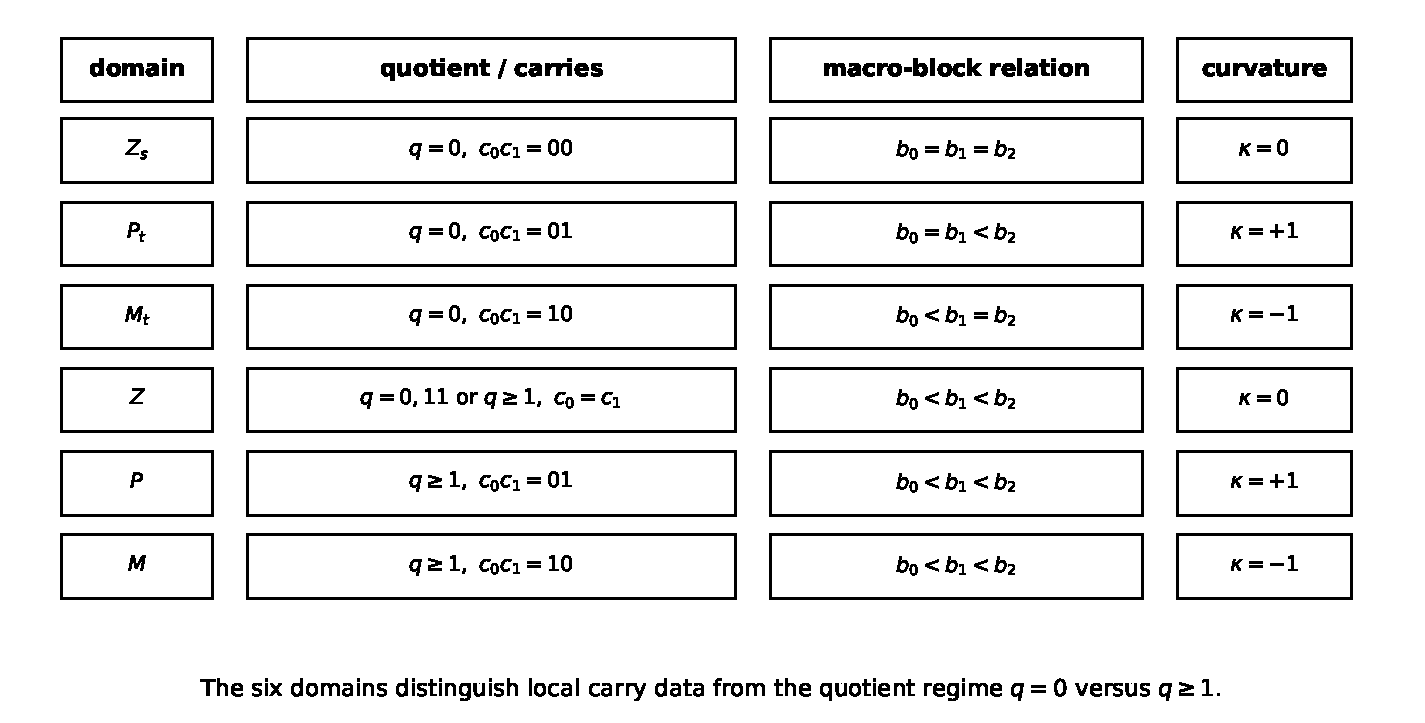
\includegraphics[width=0.92\linewidth]{FIG1_SIX_CARRY_DOMAINS.pdf}
\caption{The six physical domains. The carry pair fixes the local curvature, while the quotient regime distinguishes same/truncated cases from full ones.}
\label{fig:six-domains}
\end{figure}

\subsubsection{Worked example}\label{worked-example}

Take \(L=5\), \(K=2\), and let the first cut have local depth \(i_0=0\).
Then \(q=0\), \(r=2\), and the recurrence gives

\[
(i_0,i_1,i_2)=(0,2,4),\qquad(c_0,c_1)=(0,0).
\]

All three cutpoints lie in one macro block, so this is a \(Z_s\) window.
If that block has the unresolved role, the raw support is

\[
x_0-2x_2+x_4,
\]

which reduces to \(-2x_2+x_4\) because \(x_0=0\). This small example is
the simplest nonempty member of the stable same-block family.

\subsubsection{Lemma 3.2 --- one-point
truncation}\label{lemma-3.2-one-point-truncation}

The truncated nonzero-curvature domains differ from the corresponding
full domains by exactly one local triple:

\[
P_t
=
P\setminus\{(L-2,L-1,0)\},
\tag{3.13}
\]

\[
M_t
=
M\setminus\{(L-1,0,1)\}.
\tag{3.14}
\]

\paragraph{Proof}\label{proof-1}

For \(P\), write \(i_1-i_0=\eta\). The \(q=0\) condition gives
\(K=\eta\ge2\), whereas the full domain permits \(\eta=1\). Substituting
\(\eta=1\) into the local inequalities forces \(a=L-2\), giving
\((L-2,L-1,0)\).

For \(M\), the smallest possible \(\eta\) is \(1-L\), realized only by
\((L-1,0,1)\). In the \(q=0\) truncated realization the period condition
is \(L+\eta\ge2\), which removes precisely that point. \(\square\)

\subsection{4. Physical role projection}\label{physical-role-projection}

For a candidate window, write

\[
\chi_j=\chi(b_j)\in\{0,1\},
\qquad j=0,1,2,
\]

where \(\chi_j=1\) means that the macro block containing the \(j\)-th
cutpoint has the unresolved role \(X\). The three bits are not always
independent: when two cutpoints lie in the same macro block, their bits
must agree.

For a mask \(\chi=(\chi_0,\chi_1,\chi_2)\), define

\[
\pi_\chi(u,v,w)
=
\operatorname{red}
\left(
\chi_0x_u-2\chi_1x_v+\chi_2x_w
\right),
\tag{4.1}
\]

where \texttt{red} removes \(x_0\), combines equal depths, and deletes
zero coefficients. For a physical domain \(D\), the corresponding
\textbf{complete support set} is \(\pi_\chi(D)\).

\subsubsection{Lemma 4.1 --- exactly 34 physically realizable
domain/mask
patterns}\label{lemma-4.1-exactly-34-physically-realizable-domainmask-patterns}

For \(L\ge5\):

\begin{itemize}
\tightlist
\item
  \(Z_s\) admits \(000,111\);
\item
  \(P_t\) admits \(000,001,110,111\);
\item
  \(M_t\) admits \(000,100,011,111\);
\item
  each of \(Z,P,M\) admits all eight binary masks.
\end{itemize}

Hence

\[
2+4+4+8+8+8=34.
\tag{4.2}
\]

Every one of these \(34\) patterns has a geometric realization for
\(L\ge5\).

\paragraph{Proof}\label{proof-2}

In \(Z_s\), all three cutpoints lie in the same macro block, so all
three occurrence bits agree. In \(P_t\), the first two cutpoints share a
block, hence \(\chi_0=\chi_1\); in \(M_t\), the last two share a block,
hence \(\chi_1=\chi_2\). In the full domains \(Z,P,M\), the three
cutpoints can lie in three distinct macro blocks, so every mask is
realizable. Explicit interior points exist for each domain once
\(L\ge5\). \(\square\)

The number \(34\) counts physical \textbf{domain/mask cases}. The number
\(19\) below counts equality classes of \textbf{complete support sets}.
These are different objects.

\subsubsection{Lemma 4.2 --- truncation and support
rescue}\label{lemma-4.2-truncation-and-support-rescue}

The truncated nonzero-curvature domains are

\[
P_t=P\setminus\{p^+\},
\qquad
p^+=(L-2,L-1,0),
\tag{4.3}
\]

and

\[
M_t=M\setminus\{p^-\},
\qquad
p^-=(L-1,0,1).
\tag{4.4}
\]

Under the physically realizable masks, the deleted point changes the
complete support set in exactly one case on each side:

\[
\pi_{110}(P_t)
=
\pi_{110}(P)
\setminus
\{x_{L-2}-2x_{L-1}\},
\tag{4.5}
\]

\[
\pi_{011}(M_t)
=
\pi_{011}(M)
\setminus
\{x_1\}.
\tag{4.6}
\]

All other nonempty truncated support images agree with their full-domain
counterparts.

\paragraph{Proof}\label{proof-3}

For the positive side, \(P_t=P\setminus\{p^+\}\).

\begin{itemize}
\item
  Under mask \(001\), \[
  \pi_{001}(p^+)=x_0=0,
  \] and \(0\) is already realized inside \(P_t\), for example by
  \((L-4,L-2,0)\).
\item
  Under mask \(111\), \[
  \pi_{111}(p^+)=x_{L-2}-2x_{L-1}.
  \] The point \[
  (0,L-1,L-2)\in P_t
  \] gives the same reduced signature.
\item
  Under mask \(110\), the same deleted point gives \(x_{L-2}-2x_{L-1}\).
  In a \(110\) projection, the coefficient \(-2\) fixes \(v=L-1\) and
  the coefficient \(+1\) fixes \(u=L-2\); hence any realization is
  \(p^+\) itself. No rescue is possible.
\end{itemize}

For the negative side, \(M_t=M\setminus\{p^-\}\).

\begin{itemize}
\item
  Under mask \(100\), \[
  \pi_{100}(p^-)=x_{L-1},
  \] which is already realized by \((L-1,1,3)\in M_t\).
\item
  Under mask \(111\), \[
  \pi_{111}(p^-)=x_{L-1}+x_1,
  \] and \[
  (1,0,L-1)\in M_t
  \] gives the same reduced signature.
\item
  Under mask \(011\), \(\pi_{011}(p^-)=x_1\). Producing this singleton
  forces \(v=0\) and \(w=1\); the domain equation then forces \(u=L-1\),
  so the deleted point is the unique realization.
\end{itemize}

Thus each truncated side contributes exactly one genuinely new support
set. \(\square\)

\subsubsection{4.1 Outer reversal}\label{outer-reversal}

For each full domain \(D\in\{Z,P,M\}\), outer reversal

\[
(u,v,w)\longmapsto(w,v,u)
\tag{4.7}
\]

preserves \(D\). Therefore

\[
\pi_{001}(D)=\pi_{100}(D),
\qquad
\pi_{011}(D)=\pi_{110}(D).
\tag{4.8}
\]

All \(000\) cases give the same empty support set

\[
E=\{0\}.
\tag{4.9}
\]

After removing \(E\), each full domain therefore contributes at most
five nonempty support types. The same-block domain contributes one
additional all-active type, and Lemma 4.2 contributes one additional
truncated centre--outer type on each nonzero-curvature side. Hence the
quotient has at most

\[
1+1+5+(5+1)+(5+1)=19
\tag{4.10}
\]

classes. Section 5 proves that all nineteen are distinct.

\subsection{5. The nineteen support
families}\label{the-nineteen-support-families}

To avoid overloading the domain name \(M\), use the following
support-type abbreviations:

\[
O:x_u,\qquad
C:-2x_v,\qquad
CO:x_u-2x_v,
\]

\[
OO:x_u+x_w,\qquad
A:x_u-2x_v+x_w,
\tag{5.1}
\]

up to outer reversal.

The nineteen stable families and their cardinalities are:

{\def\LTcaptype{none} % do not increment counter
\begin{longtable}[]{@{}
  >{\raggedright\arraybackslash}p{(\linewidth - 4\tabcolsep) * \real{0.1667}}
  >{\raggedright\arraybackslash}p{(\linewidth - 4\tabcolsep) * \real{0.5417}}
  >{\raggedleft\arraybackslash}p{(\linewidth - 4\tabcolsep) * \real{0.2917}}@{}}
\toprule\noalign{}
\begin{minipage}[b]{\linewidth}\raggedright
family
\end{minipage} & \begin{minipage}[b]{\linewidth}\raggedright
description
\end{minipage} & \begin{minipage}[b]{\linewidth}\raggedleft
exact cardinality
\end{minipage} \\
\midrule\noalign{}
\endhead
\bottomrule\noalign{}
\endlastfoot
\(E\) & empty support & \(1\) \\
\(Z_s\)-A & same-block zero-curvature, all active &
\(\lfloor(L-3)^2/4\rfloor\) \\
Z-O & zero curvature, one outer & \(L\) \\
Z-C & zero curvature, centre & \(L\) \\
Z-CO & zero curvature, centre + one outer & \(\lceil L^2/2\rceil\) \\
Z-OO & zero curvature, both outers & \(\lfloor(L+1)^2/4\rfloor\) \\
Z-A & zero curvature, all active & \(\lfloor(L-1)^2/4\rfloor+1\) \\
P-O & positive curvature, one outer & \(L-1\) \\
P-C & positive curvature, centre & \(\lfloor L/2\rfloor\) \\
P-CO & positive curvature, centre + outer & \(\lfloor L^2/4\rfloor\) \\
P-OO & positive curvature, both outers &
\(\binom{\lfloor L/2\rfloor+1}{2}\) \\
P-A & positive curvature, all active &
\(\binom{\lfloor L/2\rfloor+1}{2}\) \\
\(P_t\)-CO & truncated positive centre + outer &
\(\lfloor L^2/4\rfloor-1\) \\
M-O & negative curvature, one outer & \(L-1\) \\
M-C & negative curvature, centre & \(\lfloor L/2\rfloor\) \\
M-CO & negative curvature, centre + outer & \(\lfloor L^2/4\rfloor\) \\
M-OO & negative curvature, both outers &
\(\binom{\lfloor L/2\rfloor+1}{2}\) \\
M-A & negative curvature, all active &
\(\binom{\lfloor L/2\rfloor+1}{2}\) \\
\(M_t\)-CO & truncated negative centre + outer &
\(\lfloor L^2/4\rfloor-1\) \\
\end{longtable}
}

For \(L=40\), these cardinalities are

\[
1,342,40,40,800,420,381,39,20,400,210,210,399,
39,20,400,210,210,399.
\tag{5.2}
\]

Appendix A derives all formulas directly from the domain inequalities.

\subsubsection{5.1 Proof of the main
classification}\label{proof-of-the-main-classification}

\textbf{Theorem 5.1 (Theorem A).}\\
For every \(L\ge5\), the \(34\) physically realizable domain/mask
patterns quotient, under equality of complete reduced support sets, to
exactly the nineteen families in the table above.

\paragraph{Proof}\label{proof-4}

Lemma 3.1 gives the exhaustive six-domain partition. Lemma 4.1 gives
exactly \(34\) physically consistent domain/mask cases. Equation (4.8)
identifies outer-reversal pairs in each full domain, all \(000\) masks
give the single family \(E\), and Lemma 4.2 shows that each truncated
nonzero-curvature domain adds exactly one support set not already
present in its full-domain image. Thus (4.10) gives at most nineteen
classes.

It remains to show that the nineteen displayed complete support sets are
pairwise distinct. This is done symbolically in Section 5.2. Therefore
the upper bound is attained. \(\square\)

\subsubsection{5.2 Symbolic pairwise
distinctness}\label{symbolic-pairwise-distinctness}

For a reduced formal signature

\[
\sigma=\sum_{i=1}^{L-1}\alpha_i x_i,
\]

define its \textbf{depth moment}

\[
\mu(\sigma)=\sum_{i=1}^{L-1}i\alpha_i.
\tag{5.3}
\]

The one-coordinate families are explicit:

\[
Z\text{-O}=\{0,x_1,\ldots,x_{L-1}\},
\]

\[
P\text{-O}=\{0,x_1,\ldots,x_{L-2}\},
\qquad
M\text{-O}=\{x_1,\ldots,x_{L-1}\},
\tag{5.4}
\]

and

\[
Z\text{-C}=\{0,-2x_1,\ldots,-2x_{L-1}\},
\]

\[
P\text{-C}
=
\{-2x_v:\lceil L/2\rceil\le v\le L-1\},
\]

\[
M\text{-C}
=
\{0\}\cup
\{-2x_v:1\le v\le\lfloor(L-2)/2\rfloor\}.
\tag{5.5}
\]

Hence the three O-families are distinct, the three C-families are
distinct, and no O-family equals a C-family.

For the centre--outer families,

\[
\mu(Z\text{-CO})=\{-(L-1),\ldots,0\},
\tag{5.6}
\]

\[
\mu(P\text{-CO})=\{-2L+2,\ldots,-L\},
\tag{5.7}
\]

\[
\mu(M\text{-CO})=\{1,\ldots,L-1\}.
\tag{5.8}
\]

These three moment regimes are disjoint. The truncated/full pairs are
separated by the missing witnesses

\[
x_{L-2}-2x_{L-1}
\quad\text{and}\quad
x_1
\tag{5.9}
\]

from Lemma 4.2. Thus the five centre--outer families are pairwise
distinct.

For both-outer families, P-OO and M-OO are separated by moment:

\[
0\le \mu(\sigma)\le L-2
\quad(\sigma\in P\text{-OO}),
\]

whereas

\[
L\le \mu(\sigma)\le2L-2
\quad(\sigma\in M\text{-OO}).
\tag{5.10}
\]

The zero-curvature family is separated from each of them by cardinality:

\[
|Z\text{-OO}|
=
\left\lfloor\frac{(L+1)^2}{4}\right\rfloor
\ne
\binom{\lfloor L/2\rfloor+1}{2}
=
|P\text{-OO}|=|M\text{-OO}|
\tag{5.11}
\]

for every \(L\ge5\). This avoids relying on a moment endpoint that can
overlap when \(L\) is even.

For the all-active families,

\[
\mu(Z\text{-A})=\{0\},
\qquad
\mu(P\text{-A})=\{-L\},
\qquad
\mu(M\text{-A})=\{L\},
\tag{5.12}
\]

while \(Z_s\)-A also has zero moment. The latter pair is separated by
zero membership:

\[
0\in Z\text{-A},
\qquad
0\notin Z_s\text{-A}.
\tag{5.13}
\]

Moreover \(Z_s\)-A is nonempty for \(L\ge5\), since \((0,2,4)\) gives
\(-2x_2+x_4\).

Finally, the structural groups cannot coincide across types: O-families
contain only positive unary signatures; C-families only negative doubled
unary signatures; centre--outer families contain genuine \((+1,-2)\)
two-depth signatures; OO-families have no negative coefficients; and
nonzero A-families contain the second-difference \((+1,-2,+1)\)
structure. Together with (5.4)--(5.13), this gives a uniform separator
for every one of the \(\binom{19}{2}=171\) unordered family pairs.

Therefore the nineteen complete support sets are pairwise distinct for
every \(L\ge5\). \(\square\)

\subsubsection{Corollary 5.2 --- minimality under the declared
quotient}\label{corollary-5.2-minimality-under-the-declared-quotient}

For every \(L\ge5\), nineteen is minimal under the specific rule

\begin{quote}
identify two domain/mask patterns exactly when their complete reduced
support sets are equal.
\end{quote}

This is not a minimal-automaton or optimal-implementation theorem.

\subsubsection{\texorpdfstring{5.3 Small
\(L\)}{5.3 Small L}}\label{small-l}

The equality-class counts for \(L=2,3,4,5,6,7\) are

\[
9,15,19,19,19,19.
\tag{5.14}
\]

At \(L=4\), however, \(Z_s\) is empty, so the nineteen classes are not
the stable family list above. The first same-block \(K\ge2\)
configuration occurs at \(L=5\), which is the natural lower boundary of
Theorem 5.1.

\subsection{6. Relation to earlier Abelian-power
machinery}\label{relation-to-earlier-abelian-power-machinery}

The second-difference layer itself is not new. Carpi's morphism criteria
use prefix Parikh second differences with binary whole-image correction
selectors, and the template method of Currie and Rampersad organizes
Abelian-power avoidance by finite boundary corrections. Rational carry
sequences arising from Euclidean division are likewise standard
mechanical-word objects.

The distinction made here is the following partial-assignment operation:

\[
\begin{gathered}
\text{known block data}
\; + \;
\text{one unresolved occurrence mask}\\
\longrightarrow
\text{complete reduced unresolved-support family}
\end{gathered}
\]

\subsubsection{6.1 Exact comparison with Carpi's C3
condition}\label{exact-comparison-with-carpis-c3-condition}

A modern restatement of Carpi's condition C3 asserts, for suitable
proper prefixes, the existence of binary selectors \(\delta_j\)
satisfying a whole-image corrected second-difference equation. Under a
uniform length \(L\), applying the coordinate-sum functional to the
three-cutpoint specialization gives

\[
i_0-2i_1+i_2
=
L(\delta_0-2\delta_1+\delta_2).
\]

Combining this with (3.6) yields

\[
\boxed{
\delta_0-2\delta_1+\delta_2
=
c_0-c_1
=
-\kappa.
}
\tag{6.1}
\]

Thus the scalar second-difference correction is shared prior-art
territory.

However, C3 local data do not determine the quotient

\[
q=\left\lfloor K/L\right\rfloor.
\]

Fixing \(L,r,i_0\) fixes the local depths and carry pair independently
of \(q\), while changing \(q\) changes the number of complete macro
blocks crossed between cutpoints. Hence the same local C3 instance can
occur with \(q=0\) and with \(q\ge1\). In particular, local C3 data
cannot recover the distinction

\[
Z_s\ \text{versus}\ Z,
\]

nor the analogous truncated/full nonzero-curvature split.

The six admissible C3 selector triples in the arithmetic-progression
specialization therefore do not constitute the six physical domains of
Theorem 5.1.

Our positioning is deliberately narrow. We do not claim the
\((+1,-2,+1)\) algebra, whole-image correction, Euclidean carry
arithmetic, mechanical words, template sieving, or generic finite-state
reachability. The theorem established here is the explicit
\textbf{role-projected partial-assignment classification}: the six
physical domains, the physically consistent masks, the complete reduced
support sets, and their exact \(34\to19\) quotient. Historical priority
for broader surrounding machinery is left to the cited literature rather
than inferred from the form of the present proof.

\subsection{7. Exact profile-level target
feasibility}\label{exact-profile-level-target-feasibility}

The classification in Theorem 5.1 is independent of the internal
ordering of the unresolved block. Once its total Parikh profile is
fixed, however, every reduced support signature has an exact finite set
of attainable values.

Fix

\[
\rho\in\mathbb N^{|\Sigma|},
\qquad
|\rho|_1=L,
\]

and let

\[
\sigma(x)=\sum_{j=1}^m a_jx_{d_j},
\qquad
0<d_1<\cdots<d_m<L.
\tag{7.1}
\]

Define

\[
\mathcal R_\sigma(\rho)
=
\left\{
\sum_{j=1}^m a_j\Psi(w[0..d_j)):
w\in\Sigma^L,\ \Psi(w)=\rho
\right\}.
\tag{7.2}
\]

\textbf{Corollary 7.1 --- exact feasibility for one target-loaded
window.}\\
Suppose a concrete candidate window reduces, after all assigned
contributions have been absorbed into the target, to

\[
\sigma(x)=\tau.
\tag{7.3}
\]

Among unresolved block words of profile \(\rho\), the window can be
completed to an Abelian square if and only if

\[
\tau\in\mathcal R_\sigma(\rho).
\tag{7.4}
\]

In particular,

\[
\tau\notin\mathcal R_\sigma(\rho)
\quad\Longrightarrow\quad
\text{no ordering of profile }\rho\text{ makes this window an Abelian square}.
\tag{7.5}
\]

\paragraph{Proof}\label{proof-5}

For any depths \(0<d_1<\cdots<d_m<L\), integer vectors
\(y_{d_1},\ldots,y_{d_m}\) are the prefix Parikh vectors of one word of
total profile \(\rho\) exactly when

\[
|y_{d_j}|_1=d_j
\]

for every \(j\), and

\[
0\le y_{d_1}\le\cdots\le y_{d_m}\le\rho
\]

componentwise. Necessity is immediate. Conversely, the successive
differences

\[
y_{d_1},\;
y_{d_2}-y_{d_1},\ldots,\;
y_{d_m}-y_{d_{m-1}},\;
\rho-y_{d_m}
\]

are nonnegative integer profiles of the consecutive word segments, so
choosing any word with each segment profile realizes the entire chain.

Therefore \(\mathcal R_\sigma(\rho)\) is exactly the set of values taken
by \(\sigma\) over all unresolved block words of profile \(\rho\).
Equation (7.3) is the Abelian-square Parikh equation for the declared
window after the assigned terms have been moved to the target side,
giving (7.4) and (7.5). \(\square\)

This statement concerns one declared window and one unresolved profile.
It is not a certificate for the whole coding, it does not certify all
periods, and it does not turn the nineteen support families into
nineteen global constraints.

\subsection{\texorpdfstring{8. Finite subset gates and a length-\(40\)
case
study}{8. Finite subset gates and a length-40 case study}}\label{finite-subset-gates-and-a-length-40-case-study}

The support compiler is most useful inside a staged construction if
already assigned roles are certified completely before new roles are
introduced.

Let \(w\in\Gamma^\omega\) be a fixed source word and let
\(S\subseteq\Gamma\) be the set of currently assigned roles.

\subsubsection{Lemma 8.1 --- finite subset-factor
gate}\label{lemma-8.1-finite-subset-factor-gate}

Assume that

\[
\operatorname{Fact}(w)\cap S^*
\]

has bounded word length. Let \(\mathcal C_S\) be the factor-maximal
elements of this finite language under contiguous-factor containment.
Then every output factor of \(H(w)\) whose \textbf{minimal macro
support} uses only roles in \(S\), where the minimal macro support is
the shortest contiguous source factor whose coded image covers that
output factor occurs inside \(H(c)\) for some \(c\in\mathcal C_S\).
Conversely every factor of every \(H(c)\), \(c\in\mathcal C_S\), is a
genuine factor of \(H(w)\).

Therefore absence of all \(S\)-supported Abelian squares is equivalent
to checking the finitely many cover images \(H(c)\).

\paragraph{Proof}\label{proof-6}

If an output factor has minimal supporting macro factor \(u\in
\operatorname{Fact}(w)\cap S^*\), then \(u\) is contained in a
factor-maximal \(c\in\mathcal C_S\). Uniform coding preserves aligned
factor containment, so the output factor occurs in \(H(c)\). The
converse is immediate because each \(c\) is an actual source factor.
\(\square\)

If \(|c|=m\), then every square contained in \(H(c)\) has half-period at
most

\[
\left\lfloor \frac{mL}{2}\right\rfloor.
\tag{8.1}
\]

This supplies a natural finite completion bound for each assigned-only
stage.

\subsubsection{8.1 Source and prescribed
profiles}\label{source-and-prescribed-profiles}

We now illustrate the structural theory on a concrete staged coding. The
source alphabet is

\[
\Gamma=\{a,b,c,d,e,f\}
\]

with the \(3\)-uniform morphism

\[
h_6:
\quad
a\mapsto ace,\;
b\mapsto adf,\;
c\mapsto bdf,\;
d\mapsto bdc,\;
e\mapsto afe,\;
f\mapsto bce.
\tag{8.2}
\]

The source language is

\[
\operatorname{Fact}(h_6^\omega(a)).
\]

The application seeks ternary blocks of length \(40\). The prescribed
Parikh profiles are

\[
\begin{array}{c|ccc}
\text{role}&\#a&\#b&\#c\\
\hline
A&15&14&11\\
B&11&12&17\\
C&10&14&16\\
D&12&10&18\\
E&13&16&11\\
F&19&11&10.
\end{array}
\tag{8.3}
\]

They arise from a rank-one lift of the incidence matrix of the shorter
Rao--Rosenfeld coding.

\subsubsection{Proposition 8.2 --- kernel preservation under rank-one
lifting}\label{proposition-8.2-kernel-preservation-under-rank-one-lifting}

Suppose the columns of a matrix \(B\) have common nonzero sum \(L_0\),
and let

\[
B'=sB+u\mathbf 1^T,
\qquad s\ne0.
\]

Here \(\mathbf 1\) denotes the all-ones column vector of the appropriate
dimension. If the common column sum of \(B'\) is nonzero, then

\[
\ker B'=\ker B.
\]

\paragraph{Proof}\label{proof-7}

If \(Bx=0\), summing coordinates gives \(\mathbf 1^Tx=0\), and hence
\(B'x=0\). Conversely, \(B'x=0\) and the nonzero common column sum give
\(\mathbf 1^Tx=0\), after which \(sBx=0\). \(\square\)

For the application, adding \((10,10,10)^T\) to every column raises the
block length from \(10\) to \(40\) while preserving the relevant kernel.

\subsubsection{8.2 Factor-maximal subset
covers}\label{factor-maximal-subset-covers}

For the source language (8.1), independently regenerated maximal covers
include

\[
\mathcal C_{\{A,F\}}=\{faf\},
\]

\[
\mathcal C_{\{A,E,F\}}
=
\{eafea,fafea\},
\]

and

\[
\mathcal C_{\Gamma\setminus\{C\}}
=
\{eafea,\;bdfadfbdfafea,\;ebdfafeadfbdfafea\}.
\]

At \(L=40\) their natural global half-period ceilings are respectively

\[
60,\qquad100,\qquad340.
\]

These finite gates are application-specific; Lemma 8.1 is the general
statement.

\subsection{9. Upstream compatibility as a fixed support
skeleton}\label{upstream-compatibility-as-a-fixed-support-skeleton}

Fix blocks \(E,A\) with profiles

\[
\Psi(E)=(13,16,11),
\qquad
\Psi(A)=(15,14,11).
\]

Let

\[
p(i)=\Psi(E[0..i)),
\qquad
x(j)=\Psi(A[0..j)).
\]

Examining square windows that end while the \(A\)-block is being exposed
gives three exact support classes. The words \textbf{ternary},
\textbf{binary}, and \textbf{unary} refer here to the number of
unresolved prefix vectors of \(A\) that remain after the fixed
\(E\)-contribution is moved to the target side; they do not refer to the
size of the output alphabet.

\subsubsection{\texorpdfstring{Proposition 9.1 --- \(E\to A\)
decomposition}{Proposition 9.1 --- E\textbackslash to A decomposition}}\label{proposition-9.1-eto-a-decomposition}

For the endpoint \(n=40+m\), the constraints are

\[
\begin{array}{c|c|c}
\text{class}&\text{range}&\text{forbidden equality}\\
\hline
\text{ternary}&2k\le m&
x(m)-2x(m-k)+x(m-2k)=0,\\[1mm]
\text{binary}&m<2k\le2m&
x(m)-2x(m-k)=p(40)-p(40+m-2k),\\[1mm]
\text{unary}&k>m&
x(m)=\lambda_{2k-m}-2\lambda_{k-m},
\end{array}
\tag{9.1}
\]

where \(\lambda_r\) is the Parikh vector of the last \(r\) letters of
\(E\).

For \(L=40\), the raw support counts are exactly

\[
\boxed{
361\text{ ternary},
\qquad
419\text{ binary},
\qquad
380\text{ unary}.
}
\tag{9.2}
\]

The support positions are independent of \(E\); only the affine targets
move with \(E\).

Thus compatibility is a monotone fixed-profile prefix-path problem

\[
(0,0,0)\longrightarrow(15,14,11).
\]

\subsubsection{Lemma 9.2 --- depth-one suffix
obstruction}\label{lemma-9.2-depth-one-suffix-obstruction}

For \(2\le k\le20\), define

\[
d_k(E)
=
\Psi(E[41-2k..41-k))
-
\Psi(E[41-k..40)).
\]

Let

\[
\operatorname{BLOCKED}(E)
=
\{\alpha\in\Sigma:
d_k(E)=e_\alpha
\text{ for some }2\le k\le20\}.
\]

If

\[
\operatorname{BLOCKED}(E)=\Sigma,
\]

then no compatible \(A\) exists.

The criterion is sufficient, not necessary.

\subsection{10. Downstream fixed-profile reachability and
certificates}\label{downstream-fixed-profile-reachability-and-certificates}

Fix an \(A,E\) pair and leave the order of the \(F\)-block unresolved,
with

\[
\rho=\Psi(F)=(19,11,10).
\]

For a candidate \(F=f_1\cdots f_{40}\), write

\[
X_i=\Psi(f_1\cdots f_i),
\qquad
X_0=0,
\qquad
X_{40}=\rho.
\]

Every candidate Abelian-square window becomes an affine forbidden
condition

\[
\sum_i\alpha_iX_i\in T
\tag{10.1}
\]

for a finite target set \(T\) determined by assigned data.

The profile tree is

\[
\mathcal T_\rho
=
\{u\in\Sigma^{\le40}:\Psi(u)\le\rho\}.
\tag{10.2}
\]

A constraint is \textbf{closed} when its largest referenced prefix depth
has been reached.

\subsubsection{Theorem 10.1 --- path
equivalence}\label{theorem-10.1-path-equivalence}

A profile-correct \(F\)-word satisfies all compiled constraints if and
only if its root-to-leaf path in \(\mathcal T_\rho\) never enters a
first-hit blocked edge.

Hence completion is an exact reachability problem, not a property of a
particular depth-first implementation.

\begin{figure}[t]
\centering
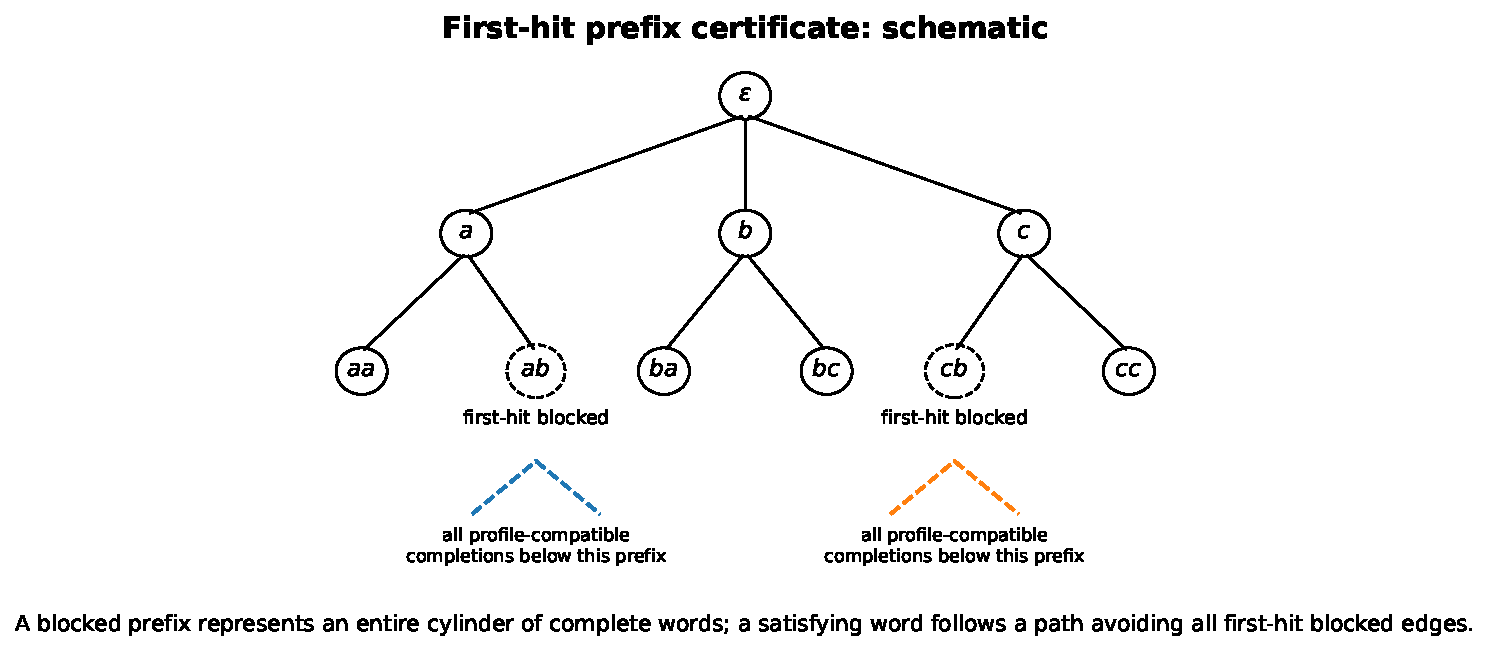
\includegraphics[width=0.88\linewidth]{FIG3_FIRST_HIT_PREFIX_TREE.pdf}
\caption{Schematic first-hit certificate. A first-hit blocked prefix removes the entire cylinder of profile-compatible complete words extending that prefix; a satisfying word is a root-to-leaf path that avoids every blocked edge.}
\label{fig:first-hit-tree}
\end{figure}

\subsubsection{10.1 First-hit certificate}\label{first-hit-certificate}

Let \(B\) be the set of bad prefixes whose parents are legal. Then \(B\)
is prefix-free. If

\[
\mathcal W_\rho
=
\{F:\Psi(F)=\rho\}
\]

and

\[
[u]_\rho
=
\{F\in\mathcal W_\rho:u\preceq F\},
\]

then the satisfying set \(\mathcal S\) obeys the exact partition

\[
\mathcal W_\rho
=
\mathcal S
\;\dot\cup\;
\mathop{\dot{\bigcup}}_{u\in B}[u]_\rho.
\tag{10.3}
\]

For \(p=\Psi(u)\),

\[
|[u]_\rho|
=
\frac{(40-|u|)!}
{(19-p_a)!(11-p_b)!(10-p_c)!}.
\tag{10.4}
\]

The total profile space is

\[
|\mathcal W_\rho|
=
\frac{40!}{19!\,11!\,10!}
=
46\,305\,405\,961\,214\,400.
\tag{10.5}
\]

An unsatisfiable instance can therefore be certified by a complete
first-hit trie whose blocked cylinders cover (10.5). An independent
checker need only verify the profile-admissible transitions and the
attached affine killers.

\subsubsection{10.2 Frontier sufficiency, and what does not
compress}\label{frontier-sufficiency-and-what-does-not-compress}

At depth \(d\), let \(A_d\) be the historical prefix depths still
referenced by an unclosed constraint. These are precisely the old prefix
values that a future affine condition may still need. The
\textbf{frontier state}

\[
S_d(u)
=
\left(
X_d(u),(X_i(u))_{i\in A_d}
\right)
\tag{10.6}
\]

is sufficient: equal frontier states have equal legal continuation
languages.

This is a correctness quotient, not a minimality theorem. In the actual
length-\(40\) system, an implementation audit finds

\[
A_d=\{1,\ldots,d\}
\]

for \(38\) of the \(40\) depths and

\[
\max_d|A_d|=38.
\]

Consecutive prefix differences recover the entire prefix word, so every
realized quotient multiplicity is \(1\). In this concrete system the
exact frontier quotient therefore coincides with the legal prefix trie
rather than compressing it.

\subsection{11. Reproducibility, scope, and
conclusion}\label{reproducibility-scope-and-conclusion}

\subsubsection{11.1 Reproducibility}\label{reproducibility}

The proof of Theorem 5.1 is symbolic. Computational artifacts are
retained as a falsification and replay layer rather than as proof
premises. Independent checkers enumerate the physical domains and masks,
reconstruct the complete support sets, verify the cardinality formulas
on finite regression ranges, and compare all family pairs. The symbolic
distinctness argument in Section 5.2, not finite enumeration, closes the
all-\(L\ge5\) claim.

For the length-\(40\) case study, the reproducibility package records
frozen scientific inputs, SHA-256 hashes, deterministic replay commands,
independent implementation checks, and literal witnesses for positive
completion cases. The project source, proof-replay material, and
computational validation artifacts are maintained at
\texttt{https://github.com/word-structures/combinatorics-on-words-research}.

\subsubsection{11.2 Scope}\label{scope}

The main simplification is a reduction in \textbf{support schemas}, not
in the number of candidate square periods. A concrete window is compiled
into

\[
\text{one support signature}
\quad+\quad
\text{one affine target}.
\]

The resulting limitations are important:

\begin{itemize}
\tightlist
\item
  the nineteen families are not nineteen automaton states;
\item
  Theorem 5.1 does not imply that checking nineteen objects certifies
  every half-period \(K\);
\item
  a support family may have many instantiated targets;
\item
  Corollary 7.1 is a single-window, fixed-profile feasibility statement;
\item
  target-loaded simultaneous completion may retain essentially the full
  prefix history, as Section 10 demonstrates;
\item
  the general Parikh second-difference and whole-image-correction
  mechanisms belong to prior work; the result here is the role-projected
  partial-assignment classification.
\end{itemize}

\subsubsection{11.3 Conclusion}\label{conclusion}

For a uniform block system with one unresolved role, the local geometry
of an Abelian-square constraint is finite and exact. Euclidean division
of the half-period gives six physical cutpoint domains. Repeated-block
consistency leaves \(34\) realizable domain/mask patterns, and equality
of complete reduced support sets collapses them to exactly \(19\) stable
families for every \(L\ge5\). Their cardinalities are explicit and their
pairwise distinctness is symbolic.

The support/target separation also provides a precise interface to
staged construction. For a prescribed unresolved-block profile, a
target-loaded window is feasible exactly when its target lies in the
reachable set of its compiled support signature. Bounded assigned-only
source factors give finite subset gates, and simultaneous target-loaded
completion can be represented as fixed-profile prefix reachability.

The broader point is structural: partial assignment need not be treated
merely as an incomplete brute-force search. It already carries a
reusable combinatorial geometry that can be isolated before concrete
targets and search order are introduced.

\section{Appendix A. Cardinality
derivations}\label{appendix-a.-cardinality-derivations}

We sketch all nineteen counts from the exact family descriptions.
Throughout, \(x_0=0\).

\subsection{A.1 Same-block family}\label{a.1-same-block-family}

For \(Z_s\)-A, each step \(\eta\ge2\) allows

\[
0\le a\le L-1-2\eta,
\]

hence \(L-2\eta\) starts. Therefore

\[
|Z_s\text{-A}|
=
\sum_{\eta=2}^{\lfloor(L-1)/2\rfloor}(L-2\eta)
=
\left\lfloor\frac{(L-3)^2}{4}\right\rfloor.
\]

The reduced signature determines \((a,\eta)\), so no further quotient
occurs.

\subsection{A.2 Zero curvature}\label{a.2-zero-curvature}

The diagonal \((d,d,d)\) exists for every \(0\le d<L\), giving

\[
|Z\text{-O}|=|Z\text{-C}|=L.
\]

For \(Z\)-CO, at fixed centre \(v\),

\[
\max(0,2v-L+1)\le w\le\min(L-1,2v),
\]

so there are

\[
2\min(v,L-1-v)+1
\]

choices. Summing gives

\[
|Z\text{-CO}|
=
\left\lceil\frac{L^2}{2}\right\rceil.
\]

For \(Z\)-OO, the unordered outer pair has equal parity. With

\[
e=\left\lceil\frac L2\right\rceil,
\qquad
o=\left\lfloor\frac L2\right\rfloor,
\]

the number of unordered pairs with repetition is

\[
\binom{e+1}{2}+\binom{o+1}{2}
=
\left\lfloor\frac{(L+1)^2}{4}\right\rfloor.
\]

For \(Z\)-A, every off-diagonal unordered outer pair gives a distinct
signature, while all \(L\) diagonal triples collapse to the zero
signature. Thus

\[
|Z\text{-A}|
=
|Z\text{-OO}|-L+1
=
\left\lfloor\frac{(L-1)^2}{4}\right\rfloor+1.
\]

\subsection{A.3 Positive curvature}\label{a.3-positive-curvature}

The relation

\[
u+w=2v-L
\]

forces

\[
\left\lceil\frac L2\right\rceil\le v\le L-1,
\qquad
0\le u+w\le L-2.
\]

Every outer depth \(0,\ldots,L-2\) occurs, so

\[
|P\text{-O}|=L-1.
\]

The possible centre depths give

\[
|P\text{-C}|=\left\lfloor\frac L2\right\rfloor.
\]

At fixed \(v\), the mixed family has

\[
0\le w\le2v-L,
\]

and the projection is injective, hence

\[
|P\text{-CO}|
=
\sum_{v=\lceil L/2\rceil}^{L-1}(2v-L+1)
=
\left\lfloor\frac{L^2}{4}\right\rfloor.
\]

Let \(n=\lfloor L/2\rfloor\). The admissible unordered outer-pair sums
have the parity of \(L\) and range below \(L\). Counting by sum gives

\[
|P\text{-OO}|
=
\sum_{j=0}^{n-1}(j+1)
=
\binom{n+1}{2}.
\]

The middle depth is uniquely determined by the outer pair, so the same
count holds for \(P\)-A:

\[
|P\text{-A}|
=
\binom{\lfloor L/2\rfloor+1}{2}.
\]

Finally, the positive truncation deletes exactly one mixed signature:

\[
|P_t\text{-CO}|
=
\left\lfloor\frac{L^2}{4}\right\rfloor-1.
\]

\subsection{A.4 Negative curvature}\label{a.4-negative-curvature}

The relation

\[
u+w=2v+L
\]

forces

\[
0\le v\le\left\lfloor\frac{L-2}{2}\right\rfloor,
\qquad
L\le u+w\le2L-2.
\]

No outer depth is \(0\), while every \(1,\ldots,L-1\) occurs, so

\[
|M\text{-O}|=L-1.
\]

The centre range, with depth \(0\) contributing the zero signature,
gives

\[
|M\text{-C}|=\left\lfloor\frac L2\right\rfloor.
\]

For the centre--outer family,

\[
2v+1\le w\le L-1,
\]

and the projection is injective. Therefore

\[
|M\text{-CO}|
=
\sum_{v=0}^{\lfloor(L-2)/2\rfloor}(L-1-2v)
=
\left\lfloor\frac{L^2}{4}\right\rfloor.
\]

Reflection

\[
(u,w)\mapsto(L-1-u,L-1-w)
\]

maps the negative-curvature outer-pair set bijectively to the positive
one, hence

\[
|M\text{-OO}|
=
|M\text{-A}|
=
\binom{\lfloor L/2\rfloor+1}{2}.
\]

The negative truncation removes exactly the signature \(x_1\), so

\[
|M_t\text{-CO}|
=
\left\lfloor\frac{L^2}{4}\right\rfloor-1.
\]

Together with \(|E|=1\), these are all nineteen formulas.

\section{Fixed-profile first-hit
counting}\label{fixed-profile-first-hit-counting}

For a fixed profile \(\rho=(\rho_1,\ldots,\rho_m)\), write

\[
\binom{n}{v}
=
\frac{n!}{\prod_j v_j!}
\]

for the multinomial coefficient when \(|v|_1=n\), where
\(|v|_1=\sum_j v_j\). A first-hit bad prefix \(u\) with profile
\(p=\Psi(u)\) eliminates exactly

\[
C_\rho(p)
=
\binom{L-|p|_1}{\rho-p}
\]

complete profile words.

If \(B\) is the first-hit antichain and \(\mathcal S\) the satisfying
set, then

\[
|\mathcal S|
+
\sum_{u\in B}C_\rho(\Psi(u))
=
\binom{L}{\rho}.
\tag{B.1}
\]

This identity is independent of search order.

More generally, if legal prefixes with identical future-relevant
frontier data are grouped into a state \(s\) of multiplicity \(N_d(s)\),
then a first-hit blocked transition to child profile \(p\) contributes

\[
N_d(s)C_\rho(p)
\]

to the blocked mass. Summing legal-leaf multiplicity and blocked mass
over all layers reproduces \(\binom{L}{\rho}\). This is an exact
quotient-DAG accounting identity. It should not be interpreted as a
guarantee of compression: in the length-\(40\) application every
realized quotient multiplicity is \(1\).

\section{Secondary finite comparison}\label{secondary-finite-comparison}

The structural theorem does not predict which assigned blocks admit a
completion. This appendix records one frozen finite comparison as an
illustration of the target-loaded feasibility problem, not as evidence
for the theorem itself.

For this section we use three explicit predicates.

\begin{itemize}
\tightlist
\item
  An \(A\)-block is \textbf{AF-compatible} if there exists a
  profile-correct \(F\)-block such that the complete \(\{A,F\}\) subset
  gate on the cover word \texttt{faf} is passed.
\item
  An \((E,A)\) pair is \textbf{AFE-completable} if there exists a
  profile-correct \(F\)-block for which the coded factor \texttt{afe}
  contains no forbidden half-period \(K\in[2,40]\).
\item
  An \((E,A)\) pair is \textbf{jointly completable} if the \textbf{same}
  \(F\)-block satisfies both conditions.
\end{itemize}

The labels \(RX\) and \(H\) refer to two frozen deterministic
populations. \(RX\) is the preregistered random-profile comparison
population. \(H\) is the frozen canonical/historical comparison
population assembled from earlier compatible constructions. Because the
latter is selected by construction, the two populations are not random
samples from a common distribution.

A preregistered deterministic quota \(Q=5000\) per \(E\)-word was
applied in the persisted enumeration order. The clean \(RX\) run
evaluated

\[
75\,111
\]

\((E,A)\) trials, representing \(36\) \(E\)-words. It produced \(137\)
AF-compatible pairs from \(17\) productive \(E\)-words, with zero
unresolved decisions. None of those \(137\) pairs was AFE-completable.

Applying the identical quota rule to the frozen \(H\) population gives:

{\def\LTcaptype{none} % do not increment counter
\begin{longtable}[]{@{}
  >{\raggedright\arraybackslash}p{(\linewidth - 10\tabcolsep) * \real{0.1304}}
  >{\raggedleft\arraybackslash}p{(\linewidth - 10\tabcolsep) * \real{0.1739}}
  >{\raggedleft\arraybackslash}p{(\linewidth - 10\tabcolsep) * \real{0.1739}}
  >{\raggedleft\arraybackslash}p{(\linewidth - 10\tabcolsep) * \real{0.1739}}
  >{\raggedleft\arraybackslash}p{(\linewidth - 10\tabcolsep) * \real{0.1739}}
  >{\raggedleft\arraybackslash}p{(\linewidth - 10\tabcolsep) * \real{0.1739}}@{}}
\toprule\noalign{}
\begin{minipage}[b]{\linewidth}\raggedright
population
\end{minipage} & \begin{minipage}[b]{\linewidth}\raggedleft
trials
\end{minipage} & \begin{minipage}[b]{\linewidth}\raggedleft
\(E\) represented
\end{minipage} & \begin{minipage}[b]{\linewidth}\raggedleft
AF-compatible
\end{minipage} & \begin{minipage}[b]{\linewidth}\raggedleft
AFE-completable
\end{minipage} & \begin{minipage}[b]{\linewidth}\raggedleft
jointly completable
\end{minipage} \\
\midrule\noalign{}
\endhead
\bottomrule\noalign{}
\endlastfoot
\(RX\) & 75,111 & 36 & 137 & 0 & 0 \\
\(H\) & 31,775 & 9 & 263 & 86 & 44 \\
\end{longtable}
}

The cleanest exact-equal-exposure strata are:

{\def\LTcaptype{none} % do not increment counter
\begin{longtable}[]{@{}lrrrrr@{}}
\toprule\noalign{}
stratum & \(E\) & trials & AF-compatible & AFE-completable & joint \\
\midrule\noalign{}
\endhead
\bottomrule\noalign{}
\endlastfoot
RX-5000-EQ & 10 & 50,000 & 63 & 0 & 0 \\
H-5000-EQ & 4 & 20,000 & 78 & 36 & 24 \\
RX-1000-EQ & 21 & 21,000 & 45 & 0 & 0 \\
H-1000-EQ & 8 & 8,000 & 40 & 19 & 0 \\
\end{longtable}
}

The AFE-completability predicate was independently recomputed on all
\(263\) quota-matched \(H\) pairs. Two implementations agreed on all
\(263\) cases: \(86\) positive, \(177\) negative, and \(0\) unresolved.
For every positive case, a separate direct checker validated one literal
\(F\)-word against the substring Parikh condition; all \(86/86\)
witnesses passed. Forty-two pairs are AFE-completable but not jointly
completable, which is a direct control that the second implementation
computes the AFE predicate rather than silently including the AF gate.

These counts are exhaustive only for the declared frozen finite
populations. They are not probability estimates, and the zero count in
\(RX\) is not a nonexistence theorem.

\section*{References}\label{references}
\addcontentsline{toc}{section}{References}

\begin{enumerate}
\def\labelenumi{\arabic{enumi}.}
\item
  A. Carpi, ``On Abelian Power-Free Morphisms,'' \emph{International
  Journal of Algebra and Computation} \textbf{3}(2) (1993), 151--168.
  doi:10.1142/S0218196793000123.
\item
  J. D. Currie and N. Rampersad, ``Fixed points avoiding Abelian
  \(k\)-powers,'' \emph{Journal of Combinatorial Theory, Series A}
  \textbf{119}(5) (2012), 942--948. doi:10.1016/j.jcta.2012.01.006.
\item
  S. Eyidoğan, H. Göral and N. Tanısalı, ``Box Progressions, Abelian
  Power-Free Morphisms and A Sieve Technique for the Template Method,''
  arXiv:2605.20504 (2026).
\item
  G. Fici and S. Puzynina, ``Abelian combinatorics on words: A survey,''
  \emph{Computer Science Review} \textbf{47} (2023), 100532.
  doi:10.1016/j.cosrev.2022.100532.
\item
  V. Keränen, ``Abelian squares are avoidable on 4 letters,'' in
  \emph{Automata, Languages and Programming}, LNCS \textbf{623} (1992),
  41--52. doi:10.1007/3-540-55719-9\_62.
\item
  M. Rao and M. Rosenfeld, ``Avoiding Two Consecutive Blocks of Same
  Size and Same Sum over \(\mathbb Z^2\),'' \emph{SIAM Journal on
  Discrete Mathematics} \textbf{32}(4) (2018), 2381--2397.
  doi:10.1137/17M1149377.
\item
  L. B. Richmond and J. Shallit, ``Counting Abelian Squares,''
  \emph{Electronic Journal of Combinatorics} \textbf{16}(1) (2009), R72.
  doi:10.37236/161.
\end{enumerate}

\end{document}
